%arara : pdflatex
\documentclass[12pt]{article}

\usepackage{../../TP0/style}

\begin{document}
\def\reportnumber{2}
\def\reporttitle{Algorithmes de Complexités temporelles linéaire O(n) et racine carrée O($\sqrt{n}$).}
%----------------------------------------------------------------------------------------
%	TITLE PAGE
%----------------------------------------------------------------------------------------


\begin{titlepage} % Suppresses displaying the page number on the title page and the subsequent page counts as page 1
	\newcommand{\HRule}{\rule{\linewidth}{0.5mm}} % Defines a new command for horizontal lines, change thickness here
	
	\center % Centre everything on the page
	
	%------------------------------------------------
	%	Headings
	%------------------------------------------------
	
	\baselineskip=2\baselineskip 
	\textsc{\LARGE Université des Sciences et de la Technologie Houari Boumediene}%\\[1cm] % Main heading such as the name of your university/college

	%------------------------------------------------
	%	Logo
	%------------------------------------------------
	
	%\vfill\vfill
	\vfill
	
\includegraphics[width=0.3\textwidth]{../style/USTHB_Logo.png}\\[1cm] % Include a department/university logo - this will require the graphicx package
	 
	%----------------------------------------------------------------------------------------
	
	\textsc{\Large Compilation}\\[0.5cm] % Major heading such as course name
	%\textsc{\large Minor Heading}\\[0.5cm] % Minor heading such as course title
	
	%------------------------------------------------
	%	Title
	%------------------------------------------------
	
	\HRule\\[0.4cm]
	\baselineskip=1.2\baselineskip 
	{\huge\bfseries Rapport de Projet \\
	 \reporttitle}\\[0.4cm] % Title of your document
	
	\HRule\\[1.5cm]
	
	%------------------------------------------------
	%	Author(s)
	%------------------------------------------------
	
	\begin{minipage}{0.4\textwidth}
		\begin{flushleft}
			\large
			\textit{Binôme: groupe 4}\\
			HOUACINE  \textsc{Naila Aziza} % Your name
			\\
			MOHAMMEDI \textsc{Haroune } % Your name
			
		\end{flushleft}
	\end{minipage}
	~
	\begin{minipage}{0.4\textwidth}
		\begin{flushright}
			\large
			\textit{Professeur}\\
			Mme. MEKAHLIA \textsc{Fatma Zohra} % Supervisor's name
		\end{flushright}
	\end{minipage}
	
	%------------------------------------------------
	%	Date
	%------------------------------------------------
	
	\vfill\vfill\vfill % Position the date 3/4 down the remaining page
	
	{\large\today} % Date, change the \today to a set date if you want to be precise
	
	
	\vfill % Push the date up 1/4 of the remaining page
	
\end{titlepage}


\section{Partie I: Algorithme 1 du test de la primalité.}

\subsection{Développement de l'algorithme qui permet de déterminer  si un nombre entier naturel n est premier (n$>$=2). }
Afin de vérifier si un nombre entier naturel "n" est premier ou pas nous allons tester s'il est divisible par un autre nombre entier naturel appartenant à l'intervalle $[2 - n]$.
Pour cela nous allons utiliser la fonction modulo qui donne le reste de la division de n par i, i variant de 1 jusqu'à n.


\begin{sql}

 Algorithme_nombre_premier1

 VAR
 i,N : entier;
 prem : booleen;
 
 DEBUT
 
	écrire("donner la valeur de N = ");
	lire(N);

	i=2;
	prem = vrai;

	tant que( i <= N-1 ET prem == vrai){

		si( N mod i == 0)
			alors 
				prem = faux;				
			sinon
				i = i + 1;
	}

	si(prem == 1)
    	alors
        	écrire("Le nombre saisi :",N,"est premier!");
    	sinon
        	écrire("Le nombre saisi :",N,"n'est pas premier! ");
 FIN. 
 
\end{sql}

\subsection{Complexité:}

\subsubsection{Calcule des complexités temporelles en notation exacte et/ou en notation asymptotique de Landau O (Grand O) de  cet  algorithme au meilleur cas, notée f1(n), et au pire cas, notée f2(n). }
Le calcule de la complexité exact de cet algorithme n'est pas possible car nous ne pouvons pas déterminer une forme générale représentant les nombres premiers.
 
\begin{enumerate}
	\item Calcule de la complexité au meilleur cas:
	\\
	Il s'agit du cas ou le nombre est égale à 2 donc la boucle n'est exécutée aucune fois, tel que :
	\\
	f1(n) = 1(=) + 1(=) + 4($<$= , - , == , et) 
	\\
	\color{blue}
	f1(n) = 6 (Opérations) $\Rightarrow$ f1(n) = O(1)
	\color{black}
	\\
	\item Calcule de la complexité au pire cas:
	\\
	Il s'agit du cas ou le nombre est premier c'est à dire le contenu de la boucle est exécuté (n-1)-2 + 1 fois = n-2 fois.
	(selon la règle : fin-debut+1)
	\\
	ce qui donne:
	\\
	f2(n) = 1(=) + 1(=) + 4($<$=,-,==,et)(n-1) + [2(mod,==)+2(+,=)](n-2) 
	\\
	\color{blue}
	f2(n) = 8n - 10 (Opérations) $\Rightarrow$ f2(n) = O(n)
	\color{black}
\end{enumerate}




\subsubsection{Calculer la complexité spatiale en notation exacte et/ou en notation asymptotique de Landau O (Grand O) de  cet  algorithme notée s(n).}



\subsection{Développement de programme correspondant avec le langage C.}


\begin{sql}
#include <stdlib.h>
#include <stdio.h>

int main()
{

	int i,N,prem;


	printf("donner la valeur de N = ");
	scanf("%d",&N);

	i=2;
	prem = 1;

	while( i <= N-1 && prem == 1){

		if( N%i == 0)
			prem = 0;
		else
			i = i + 1;
	}

	if(prem == 1)
    {
        printf("Le nombre saisi : %d est premier! \n",N);
    }
	else{
        printf("Le nombre saisi : %d n'est pas premier! \n",N);
	}


return 0;

}

\end{sql}



\subsection{Vérification par programme  si  les  nombres  n  donnés  dans  le tableau de l'énoncé (1.000.003, 2.000.003, …) sont premiers.}

Pour répondre à cette question, notre programme doit contenir une tableau tab[ ] des valeurs à tester, ainsi le programme de teste de primalité devra être exécuté pour chaque élément de ce tableau.

\subsubsection{Programme C à exécuter:}

\begin{sql}
#include <stdlib.h>
#include <stdio.h>
#include <time.h>

int main()
{
	long int i,j,prem;

	long int tab[]={1000003, 2000003, 4000037, 8000009, 16000057, 32000011, 64000031, 128000003, 256000001, 512000009,	1024000009,	2048000011};

for(j=0 ; j<12 ; j++)
{
	i=2;
	prem = 1;
	
	while( i <= tab[j]-1 && prem == 1){

		if( tab[j]%i == 0)
			prem = 0;
		else
			i = i + 1;
	}

	if(prem == 1)
    {
        printf("Le nombre saisie : %ld est premier! \n",tab[j]);
    }
	else{
        printf("Le nombre saisie : %ld n'est pas premier! \n",tab[j]);
	}
}

return 0;
}
\end{sql}

\subsubsection{Résultats de l'exécution du programme:}
\begin{sql}
Le nombre saisie : 1000003 est premier!
Le nombre saisie : 2000003 est premier!
Le nombre saisie : 4000037 est premier!
Le nombre saisie : 8000009 est premier!
Le nombre saisie : 16000057 est premier!
Le nombre saisie : 32000011 est premier!
Le nombre saisie : 64000031 est premier!
Le nombre saisie : 128000003 est premier!
Le nombre saisie : 256000001 est premier!
Le nombre saisie : 512000009 est premier!
Le nombre saisie : 1024000009 est premier!
Le nombre saisie : 2048000011 est premier!
\end{sql}

On remarque que tous les nombres données sont premiers!

\subsection{Mesure des temps d'exécution T pour les nombres n données.}

Pour mesurer le temps d'exécution du programme nous utilisons les fonctions de gestion du temps qui sont fournies dans la bibliothèque "time.h" .

\subsubsection{Programme C correspondant au calcule du temps d'exécution pour chaque valeur du tableau:}
\begin{sql}
#include <stdlib.h>
#include <stdio.h>
#include <time.h>

int main()
{
	long int i,j,prem;
	clock_t deb,fin;
	double total;

	long int tab[]={1000003, 2000003, 4000037, 8000009, 16000057, 32000011,	64000031, 128000003, 256000001,	512000009,	1024000009, 2048000011};

for(j=0 ; j<12 ; j++)
{
	deb = clock();
	
	i=2;
	prem = 1;

	while( i <= tab[j]-1 && prem == 1){

		if( tab[j]%i == 0)
			prem = 0;
		else
			i = i + 1;
	}

	fin = clock();

	if(prem == 1)
    {
        printf("Le nombre saisie : %ld est premier! \n",tab[j]);
    }
	else{
        printf("Le nombre saisie : %ld n'est pas premier! \n",tab[j]);
	}

	total = (double) (fin - deb)/CLOCKS_PER_SEC;
	printf("temps d'exécution = %lf \n",total);
}
return 0;
}
\end{sql}

\subsubsection{Résultat de l'exécution du programme:}
\begin{sql}
Le nombre saisie : 1000003 est premier!
temps d`exécution = 0.009000
Le nombre saisie : 2000003 est premier!
temps d`exécution = 0.009000
Le nombre saisie : 4000037 est premier!
temps d`exécution = 0.013000
Le nombre saisie : 8000009 est premier!
temps d`exécution = 0.026000
Le nombre saisie : 16000057 est premier!
temps d`exécution = 0.051000
Le nombre saisie : 32000011 est premier!
temps d`exécution = 0.102000
Le nombre saisie : 64000031 est premier!
temps d`exécution = 0.205000
Le nombre saisie : 128000003 est premier!
temps d`exécution = 0.411000
Le nombre saisie : 256000001 est premier!
temps d`exécution = 0.820000
Le nombre saisie : 512000009 est premier!
temps d`exécution = 1.642000
Le nombre saisie : 1024000009 est premier!
temps d`exécution = 3.289000
Le nombre saisie : 2048000011 est premier!
temps d`exécution = 6.576000
\end{sql}


\subsubsection{Remplissage du tableau:}
\color{blue}
\textrm{  }
\\
\\
\begin{tabular}{|p{3cm}||p{1.8cm}|p{1.8cm}|p{1.8cm}|p{1.8cm}|p{1.8cm}|p{1.8cm}|}
\hline
Valeur N : & 1000003 & 2000003 & 4000037 & 8000009 & 16000057  & 32000011\\
\hline
Temps d'exe : & 0.009000 & 0.009000 & 0.013000 & 0.026000 & 0.051000 & 0.102000 \\
\hline
\end{tabular}
\\
\\
\begin{tabular}{|p{3cm}||p{1.8cm}|p{1.8cm}|p{1.8cm}|p{1.8cm}|p{1.8cm}|p{1.8cm}|}
\hline
Valeur N : & 64000031 & 128000003 & 256000001 & 512000009 &  1024000009 & 2048000011\\
\hline
Temps d'exe : &  0.205000 & 0.411000 & 0.820000 & 1.642000 & 3.289000 & 6.576000 \\
\hline
\end{tabular}


\textrm{  }
\\
\color{black}



\subsection{Développement du programme de mesure du temps d'exécution du programme qui a en entrée les données de l'échantillon dans tab1 et en sortie les temps d'exécution dans tab2. }
\begin{sql}
#include <stdlib.h>
#include <stdio.h>
#include <time.h>

int main()
{
	long int i,j,prem;
	clock_t deb,fin;
	double total;

	long int tab1[]={1000003, 2000003,	4000037,	8000009,	16000057,	32000011,	64000031,
	128000003,	256000001,	512000009,	1024000009,	2048000011};

	double tab2[12];

for(j=0 ; j<12 ; j++)
{
	deb = clock();
	
	i=2;
	prem = 1;

	while( i <= tab1[j]-1 && prem == 1){

		if( tab1[j]%i == 0)
			prem = 0;
		else
			i = i + 1;
	}
	fin = clock();

	total = (double) (fin - deb)/CLOCKS_PER_SEC;
	
	tab2[j]= total ;
	printf("%lf, ", tab2[j]);
}
return 0;

}

\end{sql}

\subsection{Représentation par un graphe, Gf1(n) et Gf2(n), les variations de la fonction de la complexité temporelle correspondant au meilleur cas f1(n) et au pire cas f2(n) en fonction de n respectivement; et par un autre graphe, noté GT(n), les variations  du temps d'exécution T(n) en fonction de n.}

\subsubsection{Représentation des deux graphes Gf1 et Gf2 du meilleur et pire cas respectivement :}
Sachant que pour le meilleur cas c'est une constante et pour le pire cas le graphe aura une forme linéaire vu sa fonction.
\\
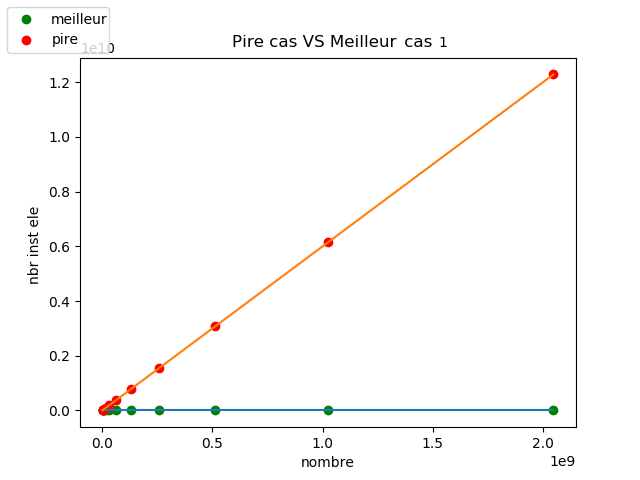
\includegraphics[width=1\textwidth]{graphe/Pire_VS_Meilleur_cas1.png}

\subsubsection{Représentation du graphe GT de la variation du temps d'exécution selon les données de teste}

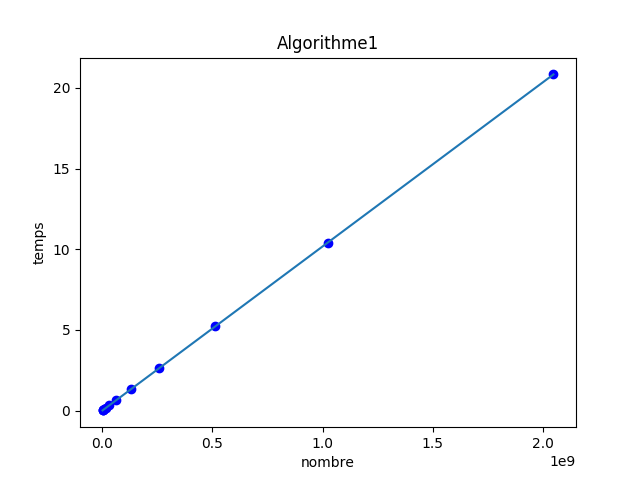
\includegraphics[width=1\textwidth]{graphe/Algorithme1.png}


\subsection{Interprétation des résultats.}
\subsubsection{Comparaison des mesure de temps d'exécution avec le pire et meilleur cas:}
\begin{enumerate}
	\item 

	\item Remarque:
	\\

\end{enumerate}

\subsubsection{Remarque est déduction d'une fonction T(n) reliant n au temps d'exécution.}

On remarque que les temps d'exécution sont approximativement doublés lorsque N est doublé.
\\

\color{blue}
Exemples:
\color{black} 
\\
N1 = $4000037  \Rightarrow  $  T1 = 0.013000
\\
N2 = $8000009 \approx 2 * N1  \Rightarrow  $  T2 = 0.026000 $\approx 2 * T1 $
\\

Aussi
\\
N1 = $128000003 \Rightarrow $  T1 = 0.411000
\\
N2 = $256000001 \approx 2 * N1 \Rightarrow $  T2 = 0.820000 $\approx 2 * T1 $
\\

On peut constater la linéarité du graphe. 
\\
\\
On en déduit que le temps d'exécution est proportionnel à N, ce que l'on peut représenter par la formule suivante
: 
\begin{center}

	$T(x*N) = x*T(N)$ pour tous $ x*N \in [1000003 - 2048000011] $	
	

(x étant la tangente d'un point sur le graphe).
\end{center}

Nous ne pouvant pas généraliser car les testes que nous avons fait n'englobent pas toutes les valeurs possibles, 
	



\subsubsection{Comparaison de la complexité théorique et expérimentale. }
\begin{enumerate}

	\item Complexité théorique:\\


	\item Complexité expérimentale:\\
	
	Nous l'avons déja calculé dans le tableau 5.3
	
	\item Nous constatons que:\\
	
	
\end{enumerate}


\section{Partie II: Algorithme 2 du test de la primalité.}

\subsection{Développement de l'algorithme qui permet de déterminer  si un nombre entier naturel n est premier (n$>$=2). }
Afin de vérifier si un nombre entier naturel "n" est premier ou pas nous allons tester s'il est divisible par un autre nombre entier naturel appartenant à l'intervalle $[2 - n/2]$.
Pour cela nous allons utiliser la fonction modulo qui donne le reste de la division de n par i, i variant de 1 jusqu'à n/2.


\begin{sql}

 Algorithme_nombre_premier2

 VAR
 i,N : entier;
 prem : booleen;
 
 DEBUT
 
	écrire("donner la valeur de N = ");
	lire(N);

	i = 2;
	prem = vrai;

	tant que( i <= (N div 2) ET prem == vrai){

		si( N mod i == 0)
			alors 
				prem = faux;				
			sinon
				i = i + 1;
	}

	si(prem == 1)
    	alors
        	écrire("Le nombre saisi :",N,"est premier!");
    	sinon
        	écrire("Le nombre saisi :",N,"n'est pas premier! ");
 FIN. 
 
\end{sql}

\subsection{Complexité:}

\subsubsection{Calcule des complexités temporelles en notation exacte et/ou en notation asymptotique de Landau O (Grand O) de  cet  algorithme au meilleur cas, notée f1(n), et au pire cas, notée f2(n). }
Le calcule de la complexité exact de cet algorithme n'est pas possible car nous ne pouvons pas déterminer une forme générale représentant les nombres premiers.
 
\begin{enumerate}
	\item Calcule de la complexité au meilleur cas:
	\\
	Il s'agit du cas ou le nombre est égale à 2 donc la boucle n'est exécutée aucune fois, tel que :
	\\
	f1(n) = 1(=) + 1(=) + 4($<$= , div , == , et) 
	\\
	\color{blue}
	f1(n) = 6 (Opérations) $\Rightarrow$ f1(n) = O(1)
	\color{black}
	\\
	\item Calcule de la complexité au pire cas:
	\\
	Il s'agit du cas ou le nombre est premier c'est à dire le contenu de la boucle est exécuté $\lfloor{\frac{n}{2}}$ - 2 + 1 fois = $\lfloor{\frac{n}{2}}$ - 1 fois.
	(selon la règle : fin-debut+1)
	\\
	ce qui donne:
	\\
	f2(n) = 1(=) + 1(=) + 4($<$=,div,==,et)($\lfloor{\frac{n}{2}}$) + [2(mod,==)+2(+,=)]($\lfloor{\frac{n}{2}}$-1) 
	\\
	\color{blue}
	f2(n) = 8$\lfloor{\frac{n}{2}}$ - 2 (Opérations) $\Rightarrow$ f2(n) = O($\lfloor{\frac{n}{2}}$) = O(n)
	\color{black}
\end{enumerate}




\subsubsection{Calculer la complexité spatiale en notation exacte et/ou en notation asymptotique de Landau O (Grand O) de  cet  algorithme notée s(n).}



\subsection{Développement de programme correspondant avec le langage C.}


\begin{sql}
#include <stdlib.h>
#include <stdio.h>

int main()
{

	int i,N,prem;

	printf("donner la valeur de N = ");
	scanf("%d",&N);

	i=2;
	prem = 1;

	while( i <= N/2 && prem == 1){

		if( N%i == 0)
			prem = 0;
		else
			i = i + 1;
	}

	if(prem == 1)
    {
        printf("Le nombre saisi : %d est premier! \n",N);
    }
	else{
        printf("Le nombre saisi : %d n'est pas premier! \n",N);
	}

return 0;
}
\end{sql}



\subsection{Vérification par programme  si  les  nombres  n  donnés  dans  le tableau de l'énoncé (1.000.003, 2.000.003, …) sont premiers.}

Pour répondre à cette question, notre programme doit contenir une tableau tab[ ] des valeurs à tester, ainsi le programme de teste de primalité devra être exécuté pour chaque élément du tableau.

\subsubsection{Programme C à exécuter:}

\begin{sql}
#include <stdlib.h>
#include <stdio.h>
#include <time.h>

int main()
{
	long int i,j,prem;

	long int tab[]={1000003, 2000003, 4000037, 8000009, 16000057, 32000011, 64000031, 128000003, 256000001, 512000009,	1024000009,	2048000011};

for(j=0 ; j<12 ; j++)
{
	i=2;
	prem = 1;
	
	while( i <= tab[j]/2 && prem == 1){

		if( tab[j]%i == 0)
			prem = 0;
		else
			i = i + 1;
	}

	if(prem == 1)
    {
        printf("Le nombre saisie : %ld est premier! \n",tab[j]);
    }
	else{
        printf("Le nombre saisie : %ld n'est pas premier! \n",tab[j]);
	}
}

return 0;
}
\end{sql}

\subsubsection{Résultats de l'exécution du programme:}
\begin{sql}
Le nombre saisie : 1000003 est premier!
Le nombre saisie : 2000003 est premier!
Le nombre saisie : 4000037 est premier!
Le nombre saisie : 8000009 est premier!
Le nombre saisie : 16000057 est premier!
Le nombre saisie : 32000011 est premier!
Le nombre saisie : 64000031 est premier!
Le nombre saisie : 128000003 est premier!
Le nombre saisie : 256000001 est premier!
Le nombre saisie : 512000009 est premier!
Le nombre saisie : 1024000009 est premier!
Le nombre saisie : 2048000011 est premier!
\end{sql}

On remarque que tous les nombre données sont premiers!

\subsection{Mesure des temps d'exécution T pour les nombres n données.}

Pour mesurer le temps d'exécution du programme nous utilisons les fonctions de gestion du temps qui sont fournies dans la bibliothèque "time.h" .

\subsubsection{Programme C correspondant au calcule du temps d'exécution pour chaque valeur du tableau:}
\begin{sql}
#include <stdlib.h>
#include <stdio.h>
#include <time.h>

int main()
{
	long int i,j,prem;
	clock_t deb,fin;
	double total;

	long int tab[]={1000003, 2000003, 4000037, 8000009, 16000057, 32000011,	64000031, 128000003, 256000001,	512000009,	1024000009, 2048000011};

for(j=0 ; j<12 ; j++)
{
	deb = clock();
	
	i=2;
	prem = 1;

	while( i <= tab[j]/2 && prem == 1){

		if( tab[j]%i == 0)
			prem = 0;
		else
			i = i + 1;
	}

	fin = clock();

	if(prem == 1)
    {
        printf("Le nombre saisie : %ld est premier! \n",tab[j]);
    }
	else{
        printf("Le nombre saisie : %ld n'est pas premier! \n",tab[j]);
	}

	total = (double) (fin - deb)/CLOCKS_PER_SEC;
	printf("temps d'exécution = %lf \n",total);
}
return 0;
}
\end{sql}

\subsubsection{Résultat de l'exécution du programme:}
\begin{sql}
Le nombre saisie : 1000003 est premier!
temps d`exécution = 0.004000
Le nombre saisie : 2000003 est premier!
temps d`exécution = 0.007000
Le nombre saisie : 4000037 est premier!
temps d`exécution = 0.009000
Le nombre saisie : 8000009 est premier!
temps d`exécution = 0.016000
Le nombre saisie : 16000057 est premier!
temps d`exécution = 0.026000
Le nombre saisie : 32000011 est premier!
temps d`exécution = 0.051000
Le nombre saisie : 64000031 est premier!
temps d`exécution = 0.102000
Le nombre saisie : 128000003 est premier!
temps d`exécution = 0.205000
Le nombre saisie : 256000001 est premier!
temps d`exécution = 0.415000
Le nombre saisie : 512000009 est premier!
temps d`exécution = 0.821000
Le nombre saisie : 1024000009 est premier!
temps d`exécution = 1.647000
Le nombre saisie : 2048000011 est premier!
temps d`exécution = 3.284000

\end{sql}


\subsubsection{Remplissage du tableau:}
\color{blue}
\textrm{  }
\\
\\
\begin{tabular}{|p{3cm}||p{1.8cm}|p{1.8cm}|p{1.8cm}|p{1.8cm}|p{1.8cm}|p{1.8cm}|}
\hline
Valeur N : & 1000003 & 2000003 & 4000037 & 8000009 & 16000057  & 32000011\\
\hline
Temps d'exe : & 0.004000 & 0.007000 & 0.009000 & 0.016000 & 0.026000 & 0.051000 \\
\hline
\end{tabular}
\\
\\
\begin{tabular}{|p{3cm}||p{1.8cm}|p{1.8cm}|p{1.8cm}|p{1.8cm}|p{1.8cm}|p{1.8cm}|}
\hline
Valeur N : & 64000031 & 128000003 & 256000001 & 512000009 &  1024000009 & 2048000011\\
\hline
Temps d'exe : &  0.102000 & 0.205000 & 0.415000 & 0.821000 &  1.647000 & 3.284000 \\
\hline
\end{tabular}


\textrm{  }
\\
\color{black}

\subsection{Développement du programme de mesure du temps d'exécution du programme qui a en entrée les données de l'échantillon dans tab1 et en sortie les temps d'exécution dans tab2. }
\begin{sql}
#include <stdlib.h>
#include <stdio.h>
#include <time.h>

int main()
{
	long int i,j,prem;
	clock_t deb,fin;
	double total;

	long int tab1[]={1000003, 2000003,	4000037,	8000009,	16000057,	32000011,	64000031,
	128000003,	256000001,	512000009,	1024000009,	2048000011};

	double tab2[12];

for(j=0 ; j<12 ; j++)
{
	deb = clock();
	
	i=2;
	prem = 1;

	while( i <= tab1[j]/2 && prem == 1){

		if( tab1[j]%i == 0)
			prem = 0;
		else
			i = i + 1;
	}
	fin = clock();

	total = (double) (fin - deb)/CLOCKS_PER_SEC;
	
	tab2[j]= total ;
	printf("%lf, ", tab2[j]);
}
return 0;

}
\end{sql}

\subsection{Représentation par un graphe, Gf1(n) et Gf2(n), les variations de la fonction de la complexité temporelle correspondant au meilleur cas f1(n) et au pire cas f2(n) en fonction de n respectivement; et par un autre graphe, noté GT(n), les variations  du temps d'exécution T(n) en fonction de n.}


\subsubsection{Représentation des deux graphes Gf1 et Gf2 du meilleur et pire cas respectivement :}
Sachant que pour le meilleur cas c'est une constante et pour le pire cas le graphe aura une forme linéaire vu sa fonction.
\\
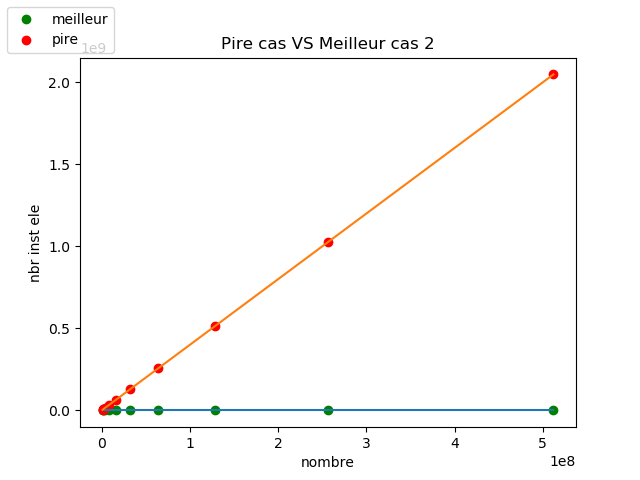
\includegraphics[width=1\textwidth]{graphe/Pire_VS_Meilleur_cas2.png}

\subsubsection{Représentation du graphe GT de la variation du temps d'exécution selon les données de teste}

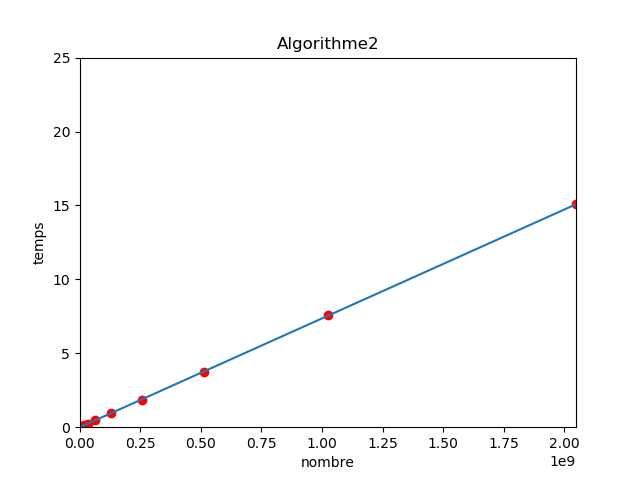
\includegraphics[width=1\textwidth]{graphe/Algorithme2.png}

\subsection{Interprétation des résultats.}
\subsubsection{Comparaison des mesure de temps d'exécution avec le pire et meilleur cas:}
\begin{enumerate}
	\item Le graphe:
	\\
	%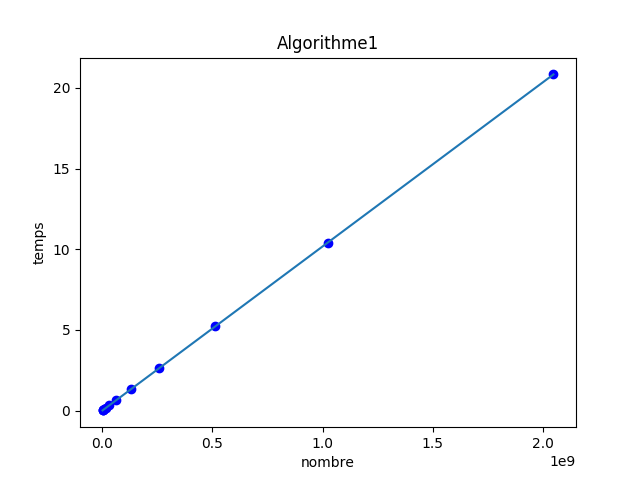
\includegraphics[width=1\textwidth]{graphe/Algorithme1.png}

	\item Remarque:
	\\
	On constate que le graphe obtenu à partir de la mesure des temps d'exécution de l'échantillon tant à ressembler au graphe du pire cas.
	\\
	Donc le graphe GT correspond au graphe du pire cas car tous les nombres de l'échantillon sont Premiers.
	
\end{enumerate}

\subsubsection{Remarque est déduction d'une fonction T(n) reliant n au temps d'exécution.}


On remarque que les temps d'exécution sont approximativement doublés lorsque N est doublé.
\\

\color{blue}
Exemples:
\color{black} 
\\
N1 = $4000037  \Rightarrow  $  T1 = 0.009000
\\
N2 = $8000009 \approx 2 * N1  \Rightarrow  $  T2 = 0.016000 $\approx 2 * T1 $
\\

Aussi
\\
N1 = $128000003 \Rightarrow $  T1 = 0.205000
\\
N2 = $256000001 \approx 2 * N1 \Rightarrow $  T2 = 0.415000 $\approx 2 * T1 $
\\

On peut constater la linéarité du graphe. 
\\
\\
On en déduit que le temps d'exécution est proportionnel à N, ce que l'on peut représenter par la formule suivante
: 
\begin{center}

	$T(x*N) = x*T(N)$ pour tous $ x*N \in [1000003 - 2048000011] $	
	

(x étant la tangente d'un point sur le graphe).
\end{center}

Nous ne pouvant pas généraliser car les testes que nous avons fait n'englobent pas toutes les valeurs possibles, 
	



\subsubsection{Comparaison de la complexité théorique et expérimentale. }

\begin{enumerate}

	\item Complexité théorique:\\
	

	\item Complexité expérimentale:\\
	
	Nous l'avons déja calculé dans le tableau 5.3
	
	\item Nous constatons que:\\
	
	
\end{enumerate}


\subsection{Comparaison des deux algorithmes précédents.}
\subsubsection{Représentation des deux graphes:}

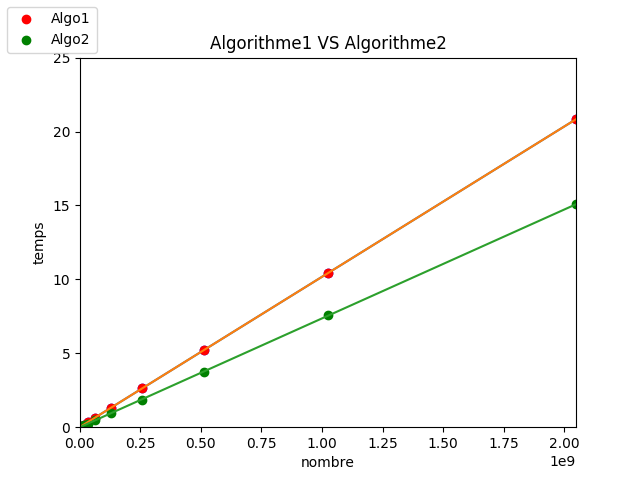
\includegraphics[width=1\textwidth]{graphe/Algorithme1_VS_Algorithme2.png}

\subsubsection{Choix de l'algorithme le plus performant:}
Il est clairement visible à travers la représentation des deux graphes ci-dessus que l'algorithme 2 ($\frac{n}{2}$) est plus rapide (temps d'exécution) que l'algorithme 1 (n).

Donc en terme de rapidité nous choisissons l'Algorithme 2.


\section{Partie III: Algorithme 3 du test de la primalité.}

\subsection{Développement de l'algorithme qui permet de déterminer  si un nombre entier naturel n est premier (n$>$=2). }
Afin de vérifier si un nombre entier naturel "n" est premier ou pas il nous allons tester s'il est divisible par un autre nombre entier naturel appartenant à l'intervalle $[2 - \sqrt(n)]$.
Pour cela nous allons utiliser la fonction modulo qui donne le reste de la division de n par i, i variant de 1 jusqu'à n.


\begin{sql}

 Algorithme_nombre_premier3

 VAR
 i,N : entier;
 prem : booleen;
 
 DEBUT
 
	écrire("donner la valeur de N = ");
	lire(N);

	i=2;
	prem = vrai;

	tant que( i <= sqrt(N) ET prem == vrai){

		si( N mod i == 0)
			alors 
				prem = faux;				
			sinon
				i = i + 1;
	}

	si(prem == 1)
    	alors
        	écrire("Le nombre saisi :",N,"est premier!");
    	sinon
        	écrire("Le nombre saisi :",N,"n'est pas premier! ");
 FIN. 
 
\end{sql}

\subsection{Complexité:}

\subsubsection{Calcule des complexités temporelles en notation exacte et/ou en notation asymptotique de Landau O (Grand O) de  cet  algorithme au meilleur cas, notée f1(n), et au pire cas, notée f2(n). }

Le calcule de la complexité exact de cet algorithme n'est pas possible car nous ne pouvons pas déterminer une forme générale représentant les nombres premiers.
 
\begin{enumerate}
	\item Calcule de la complexité au meilleur cas:
	\\
	Il s'agit du cas ou le nombre est égale à 2 donc la boucle n'est exécutée aucune fois, tel que :
	\\
	f1(n) = 1(=) + 1(=) + 4($<$= , sqrt , == , et) 
	\\
	\color{blue}
	f1(n) = 6 (Opérations) $\Rightarrow$ f1(n) = O(1)
	\color{black}
	\\
	\item Calcule de la complexité au pire cas:
	\\
	Il s'agit du cas ou le nombre est premier c'est à dire le contenu de la boucle est exécuté $\lfloor{\sqrt{n}}$ - 2 + 1 fois = $\lfloor{\sqrt{n}}$ - 1 fois.
	(selon la règle : fin-debut+1)
	\\
	ce qui donne:
	\\
	f2(n) = 1(=) + 1(=) + 4($<$=,sqrt,==,et)($\lfloor{\sqrt{n}}$) + [2(mod,==)+2(+,=)]($\lfloor{\sqrt{n}}$-1) 
	\\
	\color{blue}
	f2(n) = 8$\lfloor{\sqrt{n}}$ - 2 (Opérations) $\Rightarrow$ f2(n) = O($\lfloor{\sqrt{n}}$)= O($\sqrt{n}$)
	\color{black}
\end{enumerate}




\subsubsection{Calculer la complexité spatiale en notation exacte et/ou en notation asymptotique de Landau O (Grand O) de  cet  algorithme notée s(n).}



\subsection{Développement de programme correspondant avec le langage C.}


\begin{sql}
#include <stdlib.h>
#include <stdio.h>
#include <math.h>

int main()
{

	int i,N,prem;


	printf("donner la valeur de N = ");
	scanf("%d",&N);

	i=2;
	prem = 1;

	while( i <= sqrt(N) && prem == 1){

		if( N%i == 0)
			prem = 0;
		else
			i = i + 1;
	}

	if(prem == 1)
    {
        printf("Le nombre saisi : %d est premier! \n",N);
    }
	else{
        printf("Le nombre saisi : %d n'est pas premier! \n",N);
	}


return 0;

}

\end{sql}



\subsection{Vérification par programme  si  les  nombres  n  donnés  dans  le tableau de l'énoncé (1.000.003, 2.000.003, …) sont premiers.}

Pour répondre à cette question, notre programme doit contenir une tableau tab[] des valeurs à tester, ainsi le programme de teste de primalité devra être exécuté pour chaque élément du tableau.

\subsubsection{Programme C à exécuter:}

\begin{sql}
#include <stdlib.h>
#include <stdio.h>
#include <time.h>

int main()
{
	long int i,j,prem;

	long int tab[]={1000003, 2000003, 4000037, 8000009, 16000057, 32000011, 64000031, 128000003, 256000001, 512000009,	1024000009,	2048000011};

for(j=0 ; j<12 ; j++)
{
	i=2;
	prem = 1;
	
	while( i <= sqrt(tab[j]) && prem == 1){

		if( tab[j]%i == 0)
			prem = 0;
		else
			i = i + 1;
	}

	if(prem == 1)
    {
        printf("Le nombre saisie : %ld est premier! \n",tab[j]);
    }
	else{
        printf("Le nombre saisie : %ld n'est pas premier! \n",tab[j]);
	}
}

return 0;
}
\end{sql}

\subsubsection{Résultats de l'exécution du programme:}
\begin{sql}
Le nombre saisie : 1000003 est premier!
Le nombre saisie : 2000003 est premier!
Le nombre saisie : 4000037 est premier!
Le nombre saisie : 8000009 est premier!
Le nombre saisie : 16000057 est premier!
Le nombre saisie : 32000011 est premier!
Le nombre saisie : 64000031 est premier!
Le nombre saisie : 128000003 est premier!
Le nombre saisie : 256000001 est premier!
Le nombre saisie : 512000009 est premier!
Le nombre saisie : 1024000009 est premier!
Le nombre saisie : 2048000011 est premier!
\end{sql}

On remarque que tous les nombre données sont premiers!

\subsection{Mesure des temps d'exécution T pour les nombres n données.}

Pour mesurer le temps d'exécution du programme nous utilisons les fonctions de gestion du temps qui sont fournies dans la bibliothèque "time.h" .

\subsubsection{Programme C correspondant au calcule du temps d'exécution pour chaque valeur du tableau:}
\begin{sql}
#include <stdlib.h>
#include <stdio.h>
#include <time.h>
#include <math.h>

int main()
{
	long int i,j,prem;
	clock_t deb,fin;
	double total;

	long int tab[]={1000003, 2000003, 4000037, 8000009, 16000057, 32000011,	64000031, 128000003, 256000001,	512000009,	1024000009, 2048000011};

for(j=0 ; j<12 ; j++)
{
	deb = clock();
	i=2;
	prem = 1;

	while( i < tab[j] && prem == 1){

		if( tab[j]%i == 0)
			prem = 0;
		else
			i = i + 1;
	}

	fin = clock();

	if(prem == 1)
    {
        printf("Le nombre saisie : %ld est premier! \n",tab[j]);
    }
	else{
        printf("Le nombre saisie : %ld n'est pas premier! \n",tab[j]);
	}

	total = (double) (fin - deb)/CLOCKS_PER_SEC;
	printf("temps d'exécution = %lf \n",total);
}
return 0;
}
\end{sql}

\subsubsection{Résultat de l'exécution du programme:}
\begin{sql}
Le nombre saisie : 1000003 est premier!
temps d`exécution = 0.000000
Le nombre saisie : 2000003 est premier!
temps d`exécution = 0.000000
Le nombre saisie : 4000037 est premier!
temps d`exécution = 0.000000
Le nombre saisie : 8000009 est premier!
temps d`exécution = 0.000000
Le nombre saisie : 16000057 est premier!
temps d`exécution = 0.000000
Le nombre saisie : 32000011 est premier!
temps d`exécution = 0.001000
Le nombre saisie : 64000031 est premier!
temps d`exécution = 0.001000
Le nombre saisie : 128000003 est premier!
temps d`exécution = 0.001000
Le nombre saisie : 256000001 est premier!
temps d`exécution = 0.002000
Le nombre saisie : 512000009 est premier!
temps d`exécution = 0.002000
Le nombre saisie : 1024000009 est premier!
temps d`exécution = 0.002000
Le nombre saisie : 2048000011 est premier!
temps d`exécution = 0.003000
\end{sql}


\subsubsection{Remplissage du tableau:}
\color{blue}
\textrm{  }
\\
\\
\begin{tabular}{|p{3cm}||p{1.8cm}|p{1.8cm}|p{1.8cm}|p{1.8cm}|p{1.8cm}|p{1.8cm}|}
\hline
Valeur N : & 1000003 & 2000003 & 4000037 & 8000009 & 16000057  & 32000011\\
\hline
Temps d'exe : & 0.000000 & 0.000000 & 0.000000 & 0.000000 & 0.000000 & 0.001000 \\
\hline
\end{tabular}
\\
\\
\begin{tabular}{|p{3cm}||p{1.8cm}|p{1.8cm}|p{1.8cm}|p{1.8cm}|p{1.8cm}|p{1.8cm}|}
\hline
Valeur N : & 64000031 & 128000003 & 256000001 & 512000009 &  1024000009 & 2048000011\\
\hline
Temps d'exe : &  0.001000 & 0.001000 & 0.002000 & 0.002000 & 0.002000 & 0.003000 \\
\hline
\end{tabular}


\textrm{  }
\\
\color{black}

\subsection{Développement du programme de mesure du temps d'exécution du programme qui a en entrée les données de l'échantillon dans tab1 et en sortie les temps d'exécution dans tab2. }
\begin{sql}
#include <stdlib.h>
#include <stdio.h>
#include <time.h>

int main()
{
	long int i,j,prem;
	clock_t deb,fin;
	double total;

	long int tab1[]={1000003, 2000003,	4000037,	8000009,	16000057,	32000011,	64000031,
	128000003,	256000001,	512000009,	1024000009,	2048000011};

	double tab2[12];

for(j=0 ; j<12 ; j++)
{
	deb = clock();
	i=2;
	prem = 1;

	while( i < tab1[j] && prem == 1){

		if( tab1[j]%i == 0)
			prem = 0;
		else
			i = i + 1;
	}
	fin = clock();

	total = (double) (fin - deb)/CLOCKS_PER_SEC;
	
	tab2[j]= total ;
	printf("%lf, ", tab2[j]);
}
return 0;

}

\end{sql}

\subsection{Représentation par un graphe, Gf1(n) et Gf2(n), les variations de la fonction de la complexité temporelle correspondant au meilleur cas f1(n) et au pire cas f2(n) en fonction de n respectivement; et par un autre graphe, noté GT(n), les variations  du temps d'exécution T(n) en fonction de n.}


\subsubsection{Représentation des deux graphes Gf1 et Gf2 du meilleur et pire cas respectivement :}
Sachant que pour le meilleur cas c'est une constante et pour le pire cas le graphe aura une forme linéaire vu sa fonction.
\\
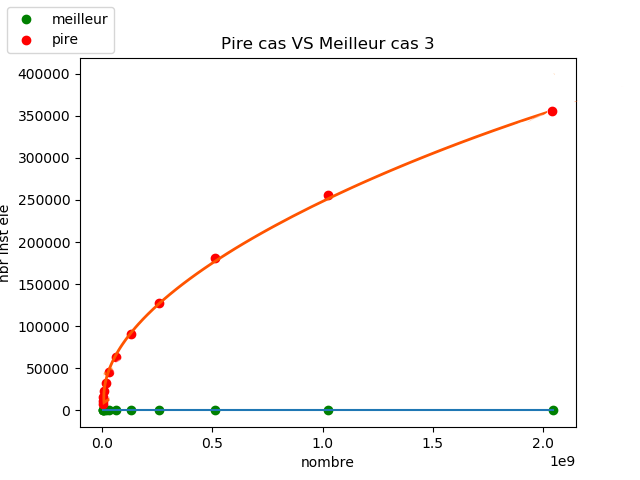
\includegraphics[width=1\textwidth]{graphe/Pire_VS_Meilleur_cas3.png}

\subsubsection{Représentation du graphe GT de la variation du temps d'exécution selon les données de teste}

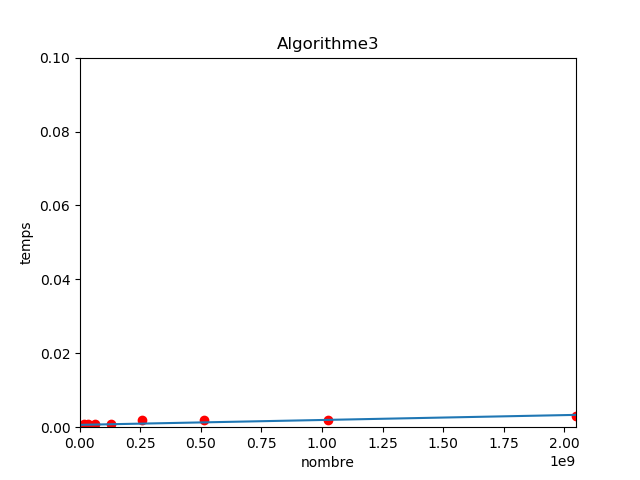
\includegraphics[width=1\textwidth]{graphe/Algorithme3.png}

\subsection{Interprétation des résultats.}
\subsubsection{Comparaison des mesure de temps d'exécution avec le pire et meilleur cas:}
\begin{enumerate}
	\item Le graphe:
	\\
	%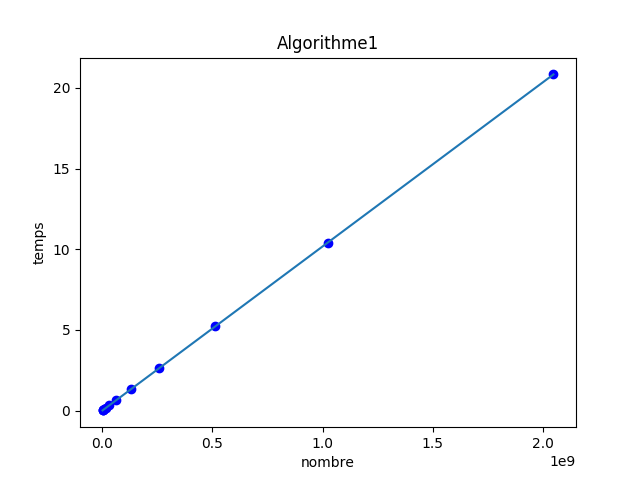
\includegraphics[width=1\textwidth]{graphe/Algorithme1.png}

	\item Remarque:
	\\
	On constate que le graphe obtenu à partir de la mesure des temps d'exécution de l'échantillon tant à ressembler au graphe du pire cas.
	\\
	Donc le graphe GT correspond au graphe du pire cas car tous les nombres de l'échantillon sont Premiers.
	
\end{enumerate}

\subsubsection{Remarque est déduction d'une fonction T(n) reliant n au temps d'exécution.}

\subsubsection{Comparaison de la complexité théorique et expérimentale. }
\begin{enumerate}

	\item Complexité théorique:\\


	\item Complexité expérimentale:\\
	
	Nous l'avons déja calculé dans le tableau 5.3
	
	\item Nous constatons que:\\
	
	
\end{enumerate}



\subsection{Comparaison des trois algorithmes précédents.}
\subsubsection{Représentation des trois graphes:}

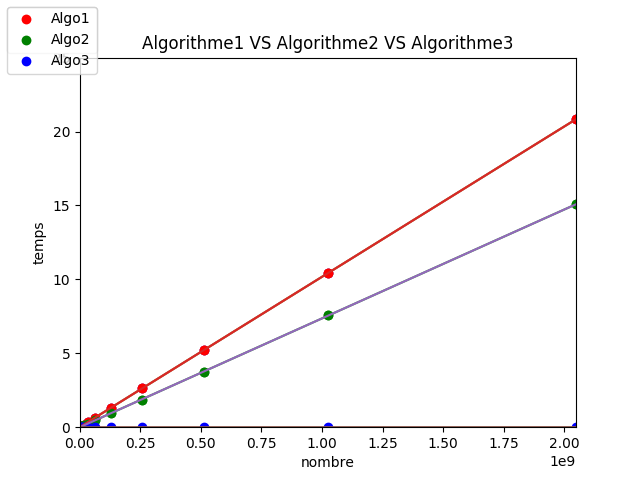
\includegraphics[width=1\textwidth]{graphe/Algorithme1_VS_Algorithme2_VS_Algorithme3.png}

\subsubsection{Choix de l'algorithme le plus performant:}
Il est clairement visible à travers la représentation des trois graphes que l'algorithme 3 ($\sqrt{n}$) est plus rapide que d'algorithme 2 ($\frac{n}{2}$) qui est lui même plus rapide que l'algorithme 1 (n).

Donc en terme de rapidité nous choisissons l'Algorithme 3.

\end{document}
